\subsection{TorCoin Mining}

Mining TorCoin requires transferring bandwidth. We introduce a novel method of
\textit{onion hashing} to prove end-to-end bandwidth transfer across a Tor
circuit.

\begin{figure}[H]
  \centering
    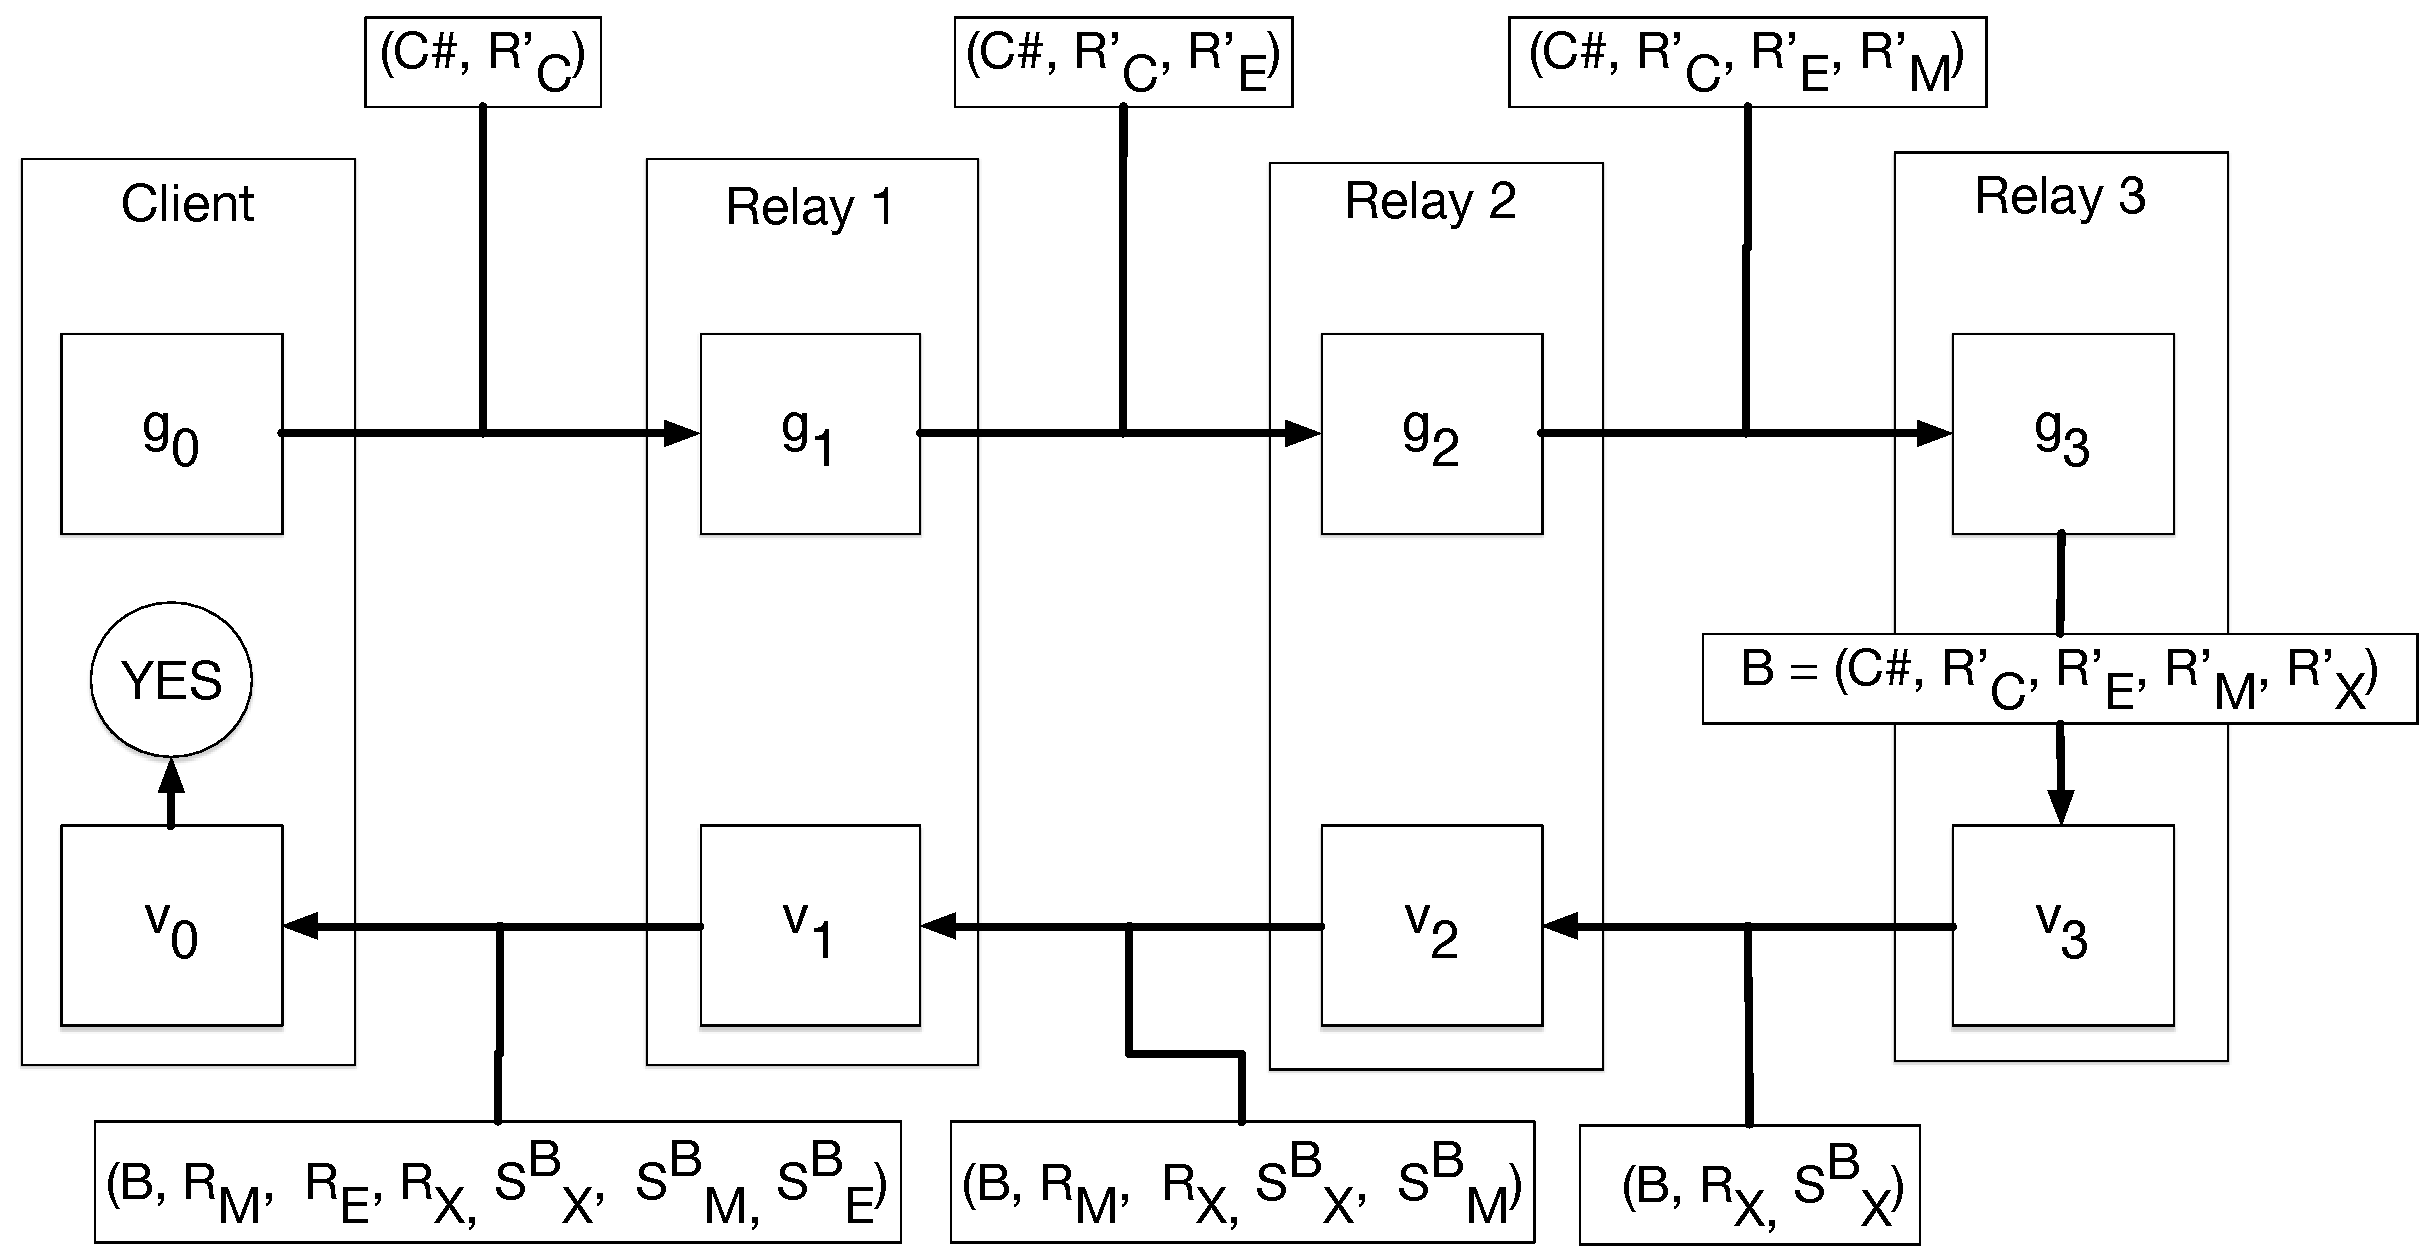
\includegraphics[scale=0.3]{torcoin_cycle.pdf}
  \caption{TorCoin Onion Hashing. Each circuit member has a generator and a 
  verifier of hash wrappers. Here we represent private keys as distinct shapes.}
\end{figure}

\subsubsection{Proof of Bandwidth}
\begin{enumerate}
\item Every $m$ Tor packets, client sends a ``TorCoin packet'' containing a hash
attempt $h$ likely to generate a TorCoin.
\item Relays sign the TorCoin packet using their own public key for that circuit, 
and send it to the next relay in the circuit.
\item The exit relay signs the packet and sends it back to the middle relay.
\item Each relay verifies the received packet by verifying the signatures. It 
then sends the packet back along the circuit. Each relay also sends its own 
TorCoin packet with its own signature for verifaction purposes.
\item The client verifies the correctness of all the signed TorCoin attempts, 
thus proving
bandwidth transfer.
\end{enumerate}

If a TorCoin is claimed, the third relay's signed packet should have the
requisite number of zeros in its lower order bits. If the claim is verified,
the client's TorCoin Wallet writes it to the blockchain, along with the
following information:

\begin{itemize}
\item Timestamp of consensus group.
\item The Hash Attempt $h$.
\item The TorCoin packets succesively signed by each relay
\item Circuit signature.
\end{itemize}

All the information necessary for verifying proof-of-bandwidth is in the
blockchain. Any interested party can then verify that the route signature is
authentic and refers to the correct group by referring to the public log.

Formally:

\begin{verbatim}
Client sends to A: h (its hash attempt)
A sends to B     : Sign(h0) = Ta
B sends to C     : Sign(Ta) = Tb
C computes       : Sign(Tb) = Tc
C sends to B     : (Tc) to verify.
B sends to A     : (Tc, Tb) to verify.
A sends to client: (Tc, Tb, Ta) to verify.
\end{verbatim}

\subsection{Security Considerations}

\subsubsection{Collusion within circuits} All honest relays and clients
enforce the TorCoin packet rate $m$. Any relays or clients that deviate from this
are reported to the assignment servers and the circuit is terminated.

\subsubsection{Enforcement of TorPath circuits} Relays know their neighbours'
IP addresses and will refuse connections from any other IP address. Even if
malicious relays connect to each other, they will not be able to sign each
other's TorCoins since they do not have the circuit signature.

\subsubsection{Compromised circuits} Any system of colluding clients and
attackers needs to control all four components of a route to mint a TorCoin
fraudulently. Even if an adversary controls up to half the network, there is a
probability of only $(\frac{1}{2})^4 = \frac{1}{16}$ that an adversary client
gets a path of three colluding relays. In practice, gaining control of half of
all Tor clients and relays would be hard for an adversary. The impact of these
compromised circuits can be further reduced by ensuring that consensus groups
expire at frequent intervals, requiring clients to change their circuits. This
limits the number of TorCoins a compromised circuit can mint.

\subsection{Drawbacks} The TorPath network is not backwards compatible with
the existing Tor network, due to the fundamental differences of route
assignment and access control, which are missing in Tor, but are necessary for
the TorPath and TorCoin schemes to work.

However, our scheme does not preclude a given physical relay or server from
running both services at the same time. They will, of course, only get paid
for the TorCoin traffic. In time, we expect that a majority of the current Tor
relay operators will switch over to the TorPath network, since TorPath has the
same security guarantees as Tor provides, while also recompensing the relay
operators for their costs.

Backwards-compatible Tor incentivization schemes like LIRA have significant
drawbacks like the usage of Eigenspeed for bandwidth measurement or the
establishment of a central bank to keep track of their tokens. These all
introduce significant infrastructure into the Tor network and may reduce
anonymity.
